\documentclass[10pt]{standalone}
\usepackage{amsmath}
\usepackage{amssymb}
\usepackage[utf8]{inputenc}
\usepackage{pgf,tikz,pgfplots}
\pgfplotsset{compat=1.15}
\usetikzlibrary{arrows}
\pagestyle{empty}

\begin{document}

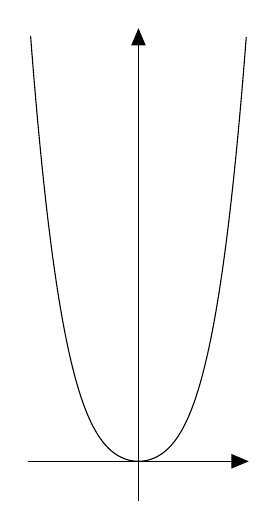
\begin{tikzpicture}[line cap=round,line join=round,>=triangle 45,x=1.0cm,y=1.0cm]
\draw[->] (-1.4,0.) -- (1.4,0.);
;
\draw[->] (0.,-0.5) -- (0.,5.5);
\draw[smooth,samples=100,domain=-1.37:1.37] plot(\x,{(\x)^(4.0)+(\x)^(2.0)});

\end{tikzpicture}
\end{document}